\chapter{Grundlagen}
\label{cha:Grundlagen}


\section{Benchmarking}

Das Vergleichen der Performanz verschiedener Systeme anhand von Messungen wird als Benchmarking bezeichnet. 
Die in diesen Messungen verwendeten Tests sind standardisiert und werden \textit{Benchmarks} genannt \cite{defi_benchmarking}.
Unter Systemen versteht man hier sowohl Hardwarekomponenten wie CPU/GPU \cite{wang2019benchmarkingtpugpucpu} oder Festplatten \cite{ssd_benchmark} als auch Software, 
beispielsweise virtuelle Maschinen (VMs) \cite{statistically_rigorous}. Um solche Benchmarks durchzuführen, werden spezielle Benchmarking-Tools eingesetzt, 
um Messungen zu ermöglichen und letztlich Vergleiche anzustellen. Das in dieser Arbeit verwendete Tool ist das Fio-Tool.

\subsection{Fio-Tool}
Das fio\footnote{flexible Input Output} \cite{axboe} Benchmarking-Tool arbeitet in der Konsole und es gibt kein UI.
Um das Programm auszuführen werden zusätzlich Parameter verwendet.
Um einen Festplattenbenchmark-Test selber durchzuführen, sieht der Command wie folgt aus:

\begin{lstlisting}[caption=Beispiel für eine Ausführung eines fio-jobs, label={lst:job}]
  ./fio --rw=write --runtime=2s --write_bw_log=mytest --name=test --size=1024m
\end{lstlisting}


\begin{center}
  \begin{table}[h!]
    \begin{tabularx}{\textwidth}{|X|X|}
      \hline
        \textbf{Parameter}& \textbf{Definition} \\ 
      \hline
      fio & Das fio Executable  \\ 
      \hline
      rw=write & Auswahl von read oder write des Tests  \\ 
      \hline
      runtime=2s & Maximale Dauer eines Tests  \\ 
      \hline
      write\_bw\_log=mytest &  Name des Logs die ausgeben werden soll   \\ 
      \hline
      name=test &  Name des Tests   \\ 
      \hline
      size=1024m & Größe der Datei für den read/write Test    \\ 
      \hline
    \end{tabularx}
    \caption{Beispiel Command zur Ausführung des Fio-Tools}
    \label{tab:1d_1_sta}
  \end{table}
\end{center}

Solche Befehle können auch in eine Datei geschrieben werden, was die .fio-Datei darstellt. 
In dieser Arbeit wird eine solche Ausführung als Job bezeichnet.
Der oben erwähnte Job testet das Random Read mit einer Laufzeit (Runtime) von 2 Sekunden und liest eine Datei mit einer Größe von 128 Mebibyte. 
Dieser Job wird nur einmal ausgeführt. Für einen wiederholten Lauf gibt es den loop-Parameter, bei dem zusätzlich die Anzahl angegeben wird, 
wie oft ein Run wiederholt werden soll. Somit ist ein Job ein abgeschlossener Durchlauf aller Runs.
Wenn der Job abgeschlossen ist und der Parameter \textit{write\_bw\_log} verwendet wurde, gibt das fio-Tool eine Log-Datei des ausgeführten Jobs aus.

\begin{lstlisting}[caption=Erste Zeilen des Logs (Bezeichnungen sind nicht im Log enthalten),label={lst:log_line_example}]
  [Time,	Bandwidth,    data direction, Blocksize,	Offset]
  0, 	    59782,        0,		            4096,		    0
  0, 	    54353,        0,		            4096,		    0
  1, 	    45545,        0,		            4096,		    0
\end{lstlisting}

Time für die Zeit in Millisekunden (ms) die verlaufen ist, Bandwidth für die
Bandbreitengeschwindigkeit in Kibibyte/s, der dritte Wert für die data direction,
 ob gelesen (= 0) oder geschrieben (= 1) wurde und ein Blocksize und
ein Offset. Die Logdaten selbst könne über 10.000 Zeilen umfassen und sind
daher schwer lesbar. Das später vorgestellte Tool wird diese Logs/Jobs auswerten.

\subsection{Warmup und stationärer Zustand}
Der stationärer Zustand ist ein Muster, das sich mit der Zeit wiederholt und bei dem das Verhalten in einem Zeitraum von der 
gleichen Natur ist wie in jedem anderen Zeitraum \cite{transient_state_definition}. Um zu ermitteln,
wann der stationäre Zustand eingetreten ist, sind stabile Messwerte erforderlich.

Bevor aber der stationäre Zustand erfolgt, ist ein Warmup erforderlich.
Dieser Warmup wird auch als transiente Zustand bezeichnet.
Ein transientes Verhalten beschreibt jene Veränderungen, bei denen sich der Charakter des Systems im Laufe der Zeit verändert \cite{transient_state_definition}.

Bei Hardware oder Software ist anfangs wiederholtes testen notwendig, um
sie analysieren zu können. 
Ein Beispiel wo die Hardware einen Warmup braucht sind die Caches beim Festplattenbenchmarking \cite{nine-year-of-bench}
Erst nach diesen Warm-ups wird der
stationäre Zustand der Performanz (engl. steady state of peak performance)
erreicht.

Hindernisse bei den Messungen in Benchmarking sind nicht-deterministische Faktoren.
Beispielsweise führt das wiederholte Lesen oder Schreiben derselben Datei auf demselben System im Durchschnitt nicht zu einer konstanten Bandbreitengeschwindigkeit, 
sondern zeigt stets Abweichungen. 
Mögliche Ursachen hierfür können unter anderem unterschiedliche CPU-Temperaturen, CPU-Scaling oder parallele Prozessierung sein \cite{statistically_rigorous}. 
Das Tool fio arbeitet dabei nicht ausschließlich mit einem Thread, sondern nutzt Multithreading, was ebenfalls nicht-deterministische Zustände hervorrufen kann. 
Zusätzlich beeinflussen auch Cache-Zustände die Messungen, abhängig davon, ob diese leer oder bereits gefüllt sind. Hintergrundprozesse, 
sowohl essentielle (z. B. Daemons) als auch nicht-essentielle Prozesse, 
können ebenfalls Schwankungen in der Geschwindigkeit verursachen \cite{nine-year-of-bench}.
Da der Nichtdeterminismus Schwankungen in den Messungen verursacht, müssen diese in Betracht gezogen werden.

Da sich die Geschwindigkeit nie konstant einem Wert nähert, sondern stets
abweicht, soll das Analysetool in Zukunft mit statistischen Tests mit einer zusätzlichen Fehlerrate den stationären
Zustand ermitteln und dabei den Nichtdeterminismus berücksichtigen.

Doch die Auswahl der Runs aus den Tests für die Bestimmung des stationäre Zustand trägt zu einer signifikante Entscheidung bei,
 ob der transiente Zustand abgeschlossen ist.
Die Auswahl der Logs und deren Diese Auswertung können signifikante Unterschiede aufweisen, die die Evaluierung
verändern \cite{when_stop_tests}.



\section{Statistische Analyse/Tests}
Es werden verschiedene Tests verwendet um herauszufinden ob eine Änderung der Performanz vorliegt \cite{statistically_rigorous}
Die Grundgesamtheit wird ein fio-Job sein und die Stichproben werden die Iteration/Runs sein die für die Tests entnommen werden.
Diese statistische Tests werden genutzt, um zu ermitteln ob eine statistische Signifikanz zwischen den Stichproben vorhanden ist.

Wenn die statistisch Signifikanz erfüllt ist, wird die Nullhypothese ($H_0$) abgelehnt \cite{inferenzstatistik}.
Die Nullhypothese ist hier die Annahme, dass es zwischen den Logs keine Abhängigkeit besteht und zufällig entstanden sind.
Somit ist die Alternativhypothese, dass zwischen den ausgewählten Stichproben ein Zusammenhang/Abhängigkeit besteht.
Die verwendeten Tests wie der t-Test und Tests mit Konfidenzintervallen haben die Bedingung, 
dass die Stichprobe einer Normalverteilung\footnote{auch Gaußverteilung} unterliegen \cite{inferenzstatistik}. 

Das Ablehnen der Nullhypothese, obwohl diese tatsächlich zutrifft, wird als Typ-I-Fehler bezeichnet. 
Die Wahrscheinlichkeit für einen solchen Fehler wird durch $\alpha$ ausgedrückt und als Signifikanzniveau bezeichnet.
Zur Überprüfung der statistischen Signifikanz werden die p-Werte (Signifikanzwahrscheinlichkeit) aus den statistischen Tests herangezogen. 
Der p-Wert repräsentiert dabei die bedingte Wahrscheinlichkeit, 
dass die beobachteten Daten oder noch extremere Ergebnisse auftreten, unter der Annahme, dass die Nullhypothese gültig ist \cite{inferenzstatistik}.

\begin{center}
  $p = P(\text{Daten}|H_0)$
\end{center}

\section{Normalverteilung/Gaußverteilung}

Die in diesem Kontext verwendeten Tests, wie der T-Test und die Quantifizierung eines Konfidenzintervalls, setzen voraus, 
dass die zugrunde liegenden Daten einer Normalverteilung folgen \cite{inferenzstatistik}.
Die Normalverteilung ist eine Dichtefunktion, die durch ihre charakteristische Glockenform beschrieben wird. Sie wird durch zwei Parameter definiert: 
die Varianz $\sigma^2$ und den Erwartungswert $\mu$. Wenn eine Zufallsvariable $X$ normalverteilt ist, kann sie durch die folgende Formel dargestellt werden:

\begin{center}
  $X \sim N(\mu,\sigma^2)$
\end{center}

Dabei bedeutet hier das $\sim$-Symbol, dass die Zufallsvariable $X$ normalverteilt ist.
Die Funktion $N$ verwendet die eigentliche Dichtefunktion:

\begin{center}
  $f(x) = \dfrac{1}{\sqrt{2\pi\sigma^2}} \cdot e^{-\frac{(x-\mu)^2}{2\sigma^2}}$
\end{center}

Die ausgewählten Stichproben entsprechen den Runs aus einem fio-Job. 
Damit spätere statistische Tests durchgeführt werden können, wird der zentrale Grenzwertsatz herangezogen, 
um die Voraussetzung der Normalverteilung zu erfüllen.
Stichproben mit $n>30$ Messwerten erfüllen diese Bedingung, da der zentrale Grenzwertsatz besagt, 
dass eine Zufallsvariable, die sich additiv aus einer großen Anzahl beliebig verteilter und stochastisch unabhängiger Zufallsvariablen zusammensetzt, 
näherungsweise normalverteilt ist \cite{statistically_rigorous}.
Eine spezielle Form der Normalverteilung ist die Standardnormalverteilung. Für diese Verteilung gilt, dass der Erwartungswert/Populationsmittelwert $\mu=0$ und die Varianz $\sigma^2=1$ ist.


\section{Varianzanalyse - Analysis of Variance (ANOVA)}
 
Dieses Kapitel führt eine allgemeine statistische Analysetechnik ein, die als Varianzanalyse (ANOVA) bezeichnet wird \cite{Lilja_2000}. 
ANOVA unterteilt die gesamte beobachtete Variation in einer Reihe von Messungen in mehrere Komponenten.
Diese Komponenten sind SSA\footnote{SSA - Sum of Squared errors of All treatment} (auch SSB \footnote{SSB - Sum of squares between}) und SSE\footnote{SSE - Sum of Squared Errors of all observation}
 (auch SSW\footnote{SSW - Sum of squares within}).
Die SSA  ist die quadratische Abweichung der Mittelwerte vom Gesamtmittelwert und die SSE
ist die gesamte Abweichung von den Mittelwerten in den Gruppen.
Das Ziel der Komponenten ist, festzustellen, ob die beobachteten Unterschiede zwischen den Mittelwerten der einzelnen Alternativen auf tatsächliche 
Unterschiede zwischen den Alternativen zurückzuführen sind oder ob sie lediglich Messfehler sind.
Die Alternativen hier werden die Iterationen eines fio-jobs sein.
Die Varianzanalyse geht davon aus, dass die Fehler in den Messungen für die verschiedenen Alternativen
unabhängig voneinander und normalverteilt sind, was mit dem Zentralen Grenzwertsatz erfüllt ist.
Die Messwerte für das Analysetool sind I/O-Geschwindigkeiten.
Es geht weiter davon aus, dass die Varianz der Messfehler bei allen Alternativen gleicher Art sind.
Die Tabelle \ref{tab:measurements} zeigt die Vorbereitung einer Varianzanalyse für einen fio-job.

\begin{table}[h!]
  \centering
  %\resizebox{\textwidth}{!}{
  \begin{tabular}{|c|*{5}{c}|c|}
  \hline
  \textbf{Messwerte} & \multicolumn{5}{c|}{\textbf{Iterationen/Alternativen}} & \textbf{Gesamtmittelwert} \\
  \cline{2-6}
   & 1 & 2 & $\cdots$ & $j$ & $k$ & \\
  \hline
  1 & $y_{11}$ & $y_{12}$ & $\cdots$ & $y_{1j}$ & $y_{1k}$ & \\
  2 & $y_{21}$ & $y_{22}$ & $\cdots$ & $y_{2j}$ & $y_{2k}$ & \\
  $\vdots$ & $\vdots$ & $\vdots$ & $\ddots$ & $\vdots$ & $\vdots$ & \\
  $i$ & $y_{i1}$ & $y_{i2}$ & $\cdots$ & $y_{ij}$ & $y_{ik}$ & \\
  $\vdots$ & $\vdots$ & $\vdots$ & $\ddots$ & $\vdots$ & $\vdots$ & \\
  $n$ & $y_{n1}$ & $y_{n2}$ & $\cdots$ & $y_{nj}$ & $y_{nk}$ &  \\
  \hline
  Spaltenmittelwert & $\bar{y}_{\cdot1}$ & $\bar{y}_{\cdot2}$ & $\cdots$ & $\bar{y}_{\cdot j}$ & $\bar{y}_{\cdot k}$ & $\bar{y}_{\cdot \cdot}$ \\
  %Effekte & $\alpha_{\cdot 1}$ & $\alpha_{\cdot 2}$ & $\cdots$ & $\alpha_{\cdot k-1}$ & $\cdots$ & $\alpha_{\cdot k}$ \\
  \hline
  \end{tabular}
  %}
  \caption{Tabelle mit einem fio-job mit k-Iterationen und n-Messwerte für die Varianzanalyse}
  \label{tab:measurements}
\end{table}

Die hier verwendete ANOVA wird als einfaktorielle ANOVA bezeichnet.
Der Faktor ist hier die I/O-Geschwindigkeit. Wenn mehr als ein Faktor verwendet wird, wird die ANOVA auch als mehrfaktorielle ANOVA bezeichnet.
Da aber nur ein fio-job mit mehreren Iteration verglichen wird, wird die einfaktorielle ANOVA benötigt.
Für die ANOVA werden folgende Formel verwendet:

\begin{itemize}
  \item $\overline{y}_{\cdot j} = \dfrac{\sum_{i=1}^{n} y_{ij}}{n}$
  \item $\overline{y}_{\cdot \cdot} = \dfrac{\sum_{j=1}^{n} \sum_{i=1}^{n} y_{ij}}{kn}$
  \item $SSE =  \sum_{i=1}^{n} (x_i - M_X)^2$
  \item $SSA = n \sum_{j=1}^{k} (\overline{y}_{\cdot j} - \overline{y}_{\cdot \cdot})^2$
  \item $SST = SSA + SSE$
\end{itemize}


Aus den beiden Komponenten SSA und SSE ergibt sich SST.
Sie ist die Summe der Quadrate der Differenzen zwischen jeder Messung und dem Gesamtmittelwert.
Mit der Berechnung des Verhältnisses von SSA und SST, wird ausgesagt, wie viel Unterschied zwischen den Alternativen sind.
und mit dem Verhältnis von SSE und SST, wie viel Variation durch Messfehler entstanden sind.  
Hier ein Beispiel für die Berechnung der Verhältnissen:

\begin{center}
  $\dfrac{SSA}{SST} = \dfrac{0.7585}{0.8270} = 0.917$
\end{center}

\begin{center}
  $\dfrac{SSE}{SST} = \dfrac{0.0685}{0.8270} = 0.083$
\end{center}

Das bedeutet 91.7\% der gesamte Variationen in den Messwerten entstammen durch den Unterschied der Performanz und
8.3\% entstammten aus Ungenauigkeiten der Messwerte. 

\subsection{F-Test}
Um die statistische Signifikanz in ANOVA zu testen wird zusätzlich der F-Test genutzt \cite[S. 71 ff.]{Lilja_2000}.
Dieser auf der F-Verteilung\footnote{Fisher-Verteilung} basierende Test wird verwendet, um zu prüfen, ob sich zwei Varianzen signifikant unterscheiden.
Der Test lässt sich mit den Verhältnissen von SSA und SSE berechnen.
Da es sich bei dieser F-Statistik um das Verhältnis zweier Varianzen handelt, sind zwei Werte für die Freiheitsgrade erforderlich, 
einer aus dem Zähler und einer aus dem Nenner.
Die Freiheitsgrade tragen dazu bei, die erhöhte Messungenauigkeit, die bei der Analyse kleiner Stichproben auftritt, 
teilweise auszugleichen, insbesondere wenn diese Stichproben zur Schätzung bestimmter Populationsparameter ($\mu$ und $\sigma^2$) herangezogen werden sollen. \cite[S. 49]{inferenzstatistik}
Wenn dieses Verhältnis, der berechnete F-Wert, größer ist als der kritische F-Wert, der bei einem bestimmten Signifikanzniveau $\alpha$ aus der F-Verteilung erhalten wird, 
schließen wir, dass der Unterschied in den Varianzen statistisch signifikant ist. Daraus ergibt sich, 
dass es einen statistisch signifikanten Unterschied zwischen den Alternativen gibt, der über die Unterschiede aufgrund experimenteller Fehler hinausgeht.

\begin{center}
  \begin{table}[h!]
    \begin{tabularx}{\textwidth}{|X|X|X|}
      \hline
       $s^2_a = \dfrac{SSA}{k - 1} = MS_{treat}$ & $s^2_e = \dfrac{SSE}{k(n-1)} = MS_{error}$ & $F = \dfrac{s^2_a}{s^2_e}$\\ 
      \hline
    \end{tabularx}
    \caption{Berechnung des F-Wertes mit mean-square SSA und SSE}
    \label{tab:f_computing}
  \end{table}
\end{center}

Den F-Wert aus einer vorgerechneten Tabelle wird mit $F_{[1-\alpha;(k-1);k(n-1)]}$ entnommen.

\section{Konfidenzintervalle}

Ein Konfidenzintervall für den Mittelwert, abgeleitet aus diesen Stichproben, quantifiziert den Wertebereich, 
der mit einer bestimmten Wahrscheinlichkeit den tatsächlichen Populationsmittelwert einschließt \cite{statistically_rigorous}.
Das Konfidenzintervall besitzt die Bedingung, dass die Messwerte aus den Stichproben normalverteilt sind.

Um ein Konfidenzintervall zu quantifizieren werden die Messwerte verwendet um den Mittelwert zu bilden.
Der Populationsmittelwert $\mu$ wird durch den Mittelwert $\overline{x}$ von den Messungen abgeschätzt
und es wird ein Bereich $[c_1,c_2]$ mittels dem geschätzten Mittelwert berechnet.
Das Konfidenzintervall $[c_1, c_2]$ ist so definiert, dass die Wahrscheinlichkeit
wenn $\mu$ zwischen c1 und c2 liegt, gleich $1 - \alpha$ ist. $\alpha$ heißt das
Signifikanzniveau und $(1 - \alpha)$ wird als Konfidenzniveau bezeichnet.
Das Signifikanzniveau wird so festgelegt, dass die Gleichung $Pr[c_1 < \mu < c_2] = 1 -\alpha$ erfüllt ist. 
Jedoch führen große $\alpha$-Werte zu einer erhöhten Wahrscheinlichkeit, die Nullhypothese fälschlicherweise abzulehnen.

Um $c_1$ und $c_2$ zu berechnet werden die Formel verwendet:

\begin{center}
         $c_1 = \overline{x} - z_{1-\alpha/2} \dfrac{s}{\sqrt{n}}$ \\
         $c_2 = \overline{x} + z_{1-\alpha/2} \dfrac{s}{\sqrt{n}}$ 

\end{center}


\begin{center}
         $s = \sqrt{\dfrac{\sum_{i=1}^{n} (x_i - \overline{x})^2}{n-1}}$ 
\end{center}

\subsection{Paarweise Konfidenzintervall-Vergleich}

Um die verschiedenen Iterationen eines fio-Jobs miteinander zu vergleichen, werden die Konfidenzintervalle der jeweiligen Messungen verglichen \cite{statistically_rigorous}. 
Eine Methode besteht darin, zu untersuchen, ob sich die Konfidenzintervalle überlappen. 
Ist dies der Fall, kann nicht mit Sicherheit geschlossen werden, dass die beobachteten Unterschiede in den Mittelwerten nicht auf zufällige Schwankungen der Messungen zurückzuführen sind.
Überlappen sich die Konfidenzintervalle jedoch nicht, gibt es keine Hinweise darauf, 
dass kein statistisch signifikanter Unterschied vorliegt. 
Diese Methode allein ist jedoch nicht ausreichend, um einen Signifikanztest durchzuführen. 
Eine alternative Methode besteht darin, ein neues Konfidenzintervall zu bilden, das sich aus den beiden zu vergleichenden Alternativen ableitet.
 Die Berechnung dieses neuen Konfidenzintervalls erfolgt wie folgt:

\begin{center}
  \begin{table}[h!]
    \begin{tabularx}{\textwidth}{|X|X|}
      \hline
       $s_x =  \sqrt{\dfrac{s^2_1}{n_1} + \dfrac{s^2_2}{n_2}}$ & Berechne den neuen Mittelwert aus den beiden Alternativen  \\ 
      \hline
      $c_1 = \overline{x} - z_{1-\alpha/2} s_x$ & Berechne den neuen Konfidenzintervall \\
      $c_2 = \overline{x} + z_{1-\alpha/2} s_x$ & \\
      \hline
    \end{tabularx}
    \caption{Berechnung kombinierten Konfidenzintervallen}
    \label{tab:two_Iteration_Konfidenzintervall}
  \end{table}
\end{center}

Wenn das neue Konfidenzintervall Null enthält, wird beschlossen, 
dass bei dem gewählten Konfidenzniveau $\alpha$ kein statistisch signifikanter Unterschied zwischen den beiden Alternativen besteht.

\section{T-Test}
Der Begriff T-Test wird verwendet, um verschiedene Tests zu bezeichnen, die unter anderem die Verteilung der Grundgesamtheit von normalverteilten 
und unabhängigen Stichproben miteinander vergleichen \cite{inferenzstatistik}. Im Kontext dieser Arbeit bezieht sich der T-Test auf den unabhängigen, ungerichteten T-Test, 
bei dem die Erwartungswerte zweier voneinander unabhängiger Stichproben verglichen werden.
Der T-Test vergleicht die Stärke der Unterschiede zwischen den Stichproben mit der Abweichung innerhalb der Stichproben. 
Die Prüfgröße $t$ dient als Maß dafür, wie unwahrscheinlich die Nullhypothese $H_0$ ist, 
d. h. dass die Grundgesamtheit der beiden Stichproben den gleichen Erwartungswert aufweisen. 
Mit dem T-Test werden jeweils zwei unabhängige Stichproben miteinander verglichen, unter der Annahme, dass die Grundgesamtheit normalverteilt ist.
Diese Prüfgröße wird wie folgt berechnet:

\begin{center}
  $t = \dfrac{M_A-M_B}{\sqrt{\frac{\hat{S}_A^2}{n_A} + \frac{\hat{S}_B^2}{n_B}}}$
\end{center}

Wobei die Varianz wie folgt berechnet wird:

\begin{center}
  $\hat{S}_X^2 = \dfrac{n}{n-1} S_X^2 = \dfrac{n}{n-1} \cdot \dfrac{1}{n} \sum_{i=1}^n (x_i - M_X)^2 = \dfrac{1}{n-1} \sum_{i=1}^n (x_i - M_X)^2$
\end{center}

Die Nullhypothese, also die Annahme, dass die Grundgesamtheit der beiden Stichproben 
den gleichen Erwartungswert haben, wird mit dem Signifikanzniveau $\alpha$ abgelehnt, wenn gilt:

\begin{center}
  $|t| > t_{n_A + n_B - 2; \frac{\alpha}{2}}$
\end{center}

Das bedeutet, dass der ermittelte t-Wert betragsmäßig größer sein muss als der Wert der t-Verteilung mit den Freiheitsgraden
 $n+m-2$ bei einem Signifikanzniveau von $1-\frac{1}{2}\alpha$.
Die t-Verteilung ähnelt der Normalverteilung, jedoch wird die t-Verteilung besonders für kleine Stichproben herangezogen, 
da sie in diesem Fall eine genauere Abschätzung der Wahrscheinlichkeiten ermöglicht.



\section{Tukey-HSD}
Der Tukey-HSD\footnote{HSD - Honestly Significant Difference} Test wird nach der Durchführung der ANOVA angewendet und wird daher auch als Post-hoc-Test bezeichnet \cite[S. 391 ff.]{tukey_hsd_book}.
Dieser Test verwendet die studentisierte Statistik $q$ und sie ist wie folgt definiert:

\begin{center}
  $q_r = \dfrac{\overline{X}_t - \overline{X}_s}{\sqrt{\dfrac{MS_{error}}{n}}}$
\end{center}

Dabei stellen $\overline{X}_l$ und $\overline{X}_s$ den größten bzw. den kleinsten Wert aus einer Menge von Mittelwerten dar, 
und $r$ ist die Anzahl der behandelten Mittelwerten.
Wenn mehr als zwei Gruppen miteinander verglichen werden, gewinnt die Kontrolle der Typ-I-Fehlerquote an zentraler Bedeutung \cite{tukey_HSD}. 
Während die Varianzanalyse (ANOVA) dabei unterstützt, das Vorliegen eines signifikanten Effekts zu identifizieren, 
stellt die Kontrolle der Typ-I-Fehlerquote insbesondere bei der Durchführung mehrerer t-Tests über mehrere Gruppen hinweg eine Herausforderung dar.
Der Tukey-Test vergleicht die Unterschiede zwischen den Mittelwerten, 
anstatt Paare von Werten direkt zu vergleichen. Der Wert des Tukey-Tests wird ermittelt, 
indem der Absolutwert der Differenz zwischen den Mittelwerten von Paaren genommen und durch den Standardfehler des Mittelwerts ($s^2_e$) geteilt wird, 
der durch einen einfaktoriellen ANOVA-Test bestimmt wird.

Nach Abschluss einer Reihe von Vergleichen zwischen den Mittelwerten der Gruppen wird die resultierende Menge von Schlussfolgerungen 
häufig als \textit{Familie} von Schlussfolgerungen bezeichnet. Diese Familie könnte beispielsweise die folgenden Aussagen umfassen:

\begin{center}
  $\mu_1 < \mu_2$ \\
  $\mu_3 < \mu_4$ \\
  $\mu_1 < \dfrac{(\mu_3 + \mu_4)}{2}$
\end{center}

Die Wahrscheinlichkeit, dass diese Familie von Schlussfolgerungen mindestens einen Fehler vom Typ I enthält,
wird als Familienfehlerrate\footnote{Family-wise error rate - FW} bezeichnet \cite[S. 365]{tukey_hsd_book}.
Es ist entscheidend, 
die Familienfehlerrate sorgfältig zu bewerten, wenn mehrere Vergleiche durchgeführt werden,
da die Wahrscheinlichkeit des Typ-I-Fehlers
bei einer Reihe von Vergleichen höher ist als die Fehlerquote bei einem einzelnen Vergleich.


\begin{center}
  $q_{\alpha}(r, df){\sqrt{\dfrac{MS_w}{n}}} = q_{HSD}$ \\
  $\overline{M}_i - \overline{M}_j \geq q_{HSD} \iff$ \text{Nullhypothese wird abgelehnt} \\
  $\overline{M}_i - \overline{M}_j < q_{HSD} \iff$ \text{Nullhypothese wird angenommen} 
\end{center}

$M_i - M_j$ ist die Differenz des Mittelwertes zweier Stichproben $i$ und $j$.
Dabei gilt das der Mittelwert $M_i$ größer ist als $M_j$.
Für $MS_w$ gilt $MS_w = s^2_{e}$ ist der quadratische Mittelwert innerhalb und n ist die Anzahl
der Alternativen.
Um diesen Test durchzuführen werden folgende Schritte angewendet:

\begin{center}
  \begin{enumerate}
    \item Führe die ANOVA durch. 
    \item Berechne den $q_{HSD}$ Wert
    \item Wähle 2 Alternativen mit den jeweiligen Mittelwerten
    \item Berechne die Differenz deren Mittelwerte
    \item Wenn der berechnete Wert größer ist als $q_{HSD}$, ist das Ergebnis signifikant unterschiedlich 
  \end{enumerate}
\end{center}


\section{Mann-Whitney-Test}
Der Mann-Whitney-Wilcoxon-Rangsummentest \cite[130 ff.]{statistik_sozialwissenschaften} \cite{u_test} wird verwendet, um zu entscheiden, 
ob sich zwei Stichproben signifikant unterscheiden, indem den Werten Ränge zugewiesen werden. Alle Werte aus den Stichproben erhalten einen Rang,
 der aufsteigend vom kleinsten zum größten Wert vergeben wird. Die gesamte Rangsumme kann mit der folgenden Formel berechnet werden:
\begin{center}
  $R_a + R_b = \dfrac{n(n + 1)}{2}, (n = n_1 + n_2)$
\end{center}  

Dabei sind $R_a$ und $R_b$ die Rangsummen aus den jeweiligen Stichproben.
Dieser Test
hat keine Anforderungen über die Verteilung der Stichproben.
Somit ist keine Normalverteilung der Stichproben notwendig.
Für Ranggrößen $n>12$ wird eine neue Statistik $Z$ eingeführt, die nach folgender Formel berechnet wird:
\begin{center}
  \[
    z_{a} = \frac{R_{a} - \frac{1}{2}m(2m+1)}{\sqrt{\frac{1}{12}m^2(2m+1)}} \text{, }
    z_{b} = \frac{R_{b} - \frac{1}{2}m(2m+1)}{\sqrt{\frac{1}{12}m^2(2m+1)}}
  \]
\end{center}

Die Nullhypothese besagt, dass keine Änderung der Performanz vorliegt. 
Die beiden alternativen Hypothesen lauten wie folgt: Die Hypothese $H_1$ besagt, dass Run A eine höhere durchschnittliche I/O-Geschwindigkeit als Run B hatte. 
Die andere Alternativhypothese $H_2$ behauptet, dass Run B im Durchschnitt schneller war.
Unter der Nullhypothese folgt, dass die Z-Statistiken $z_a$ und $z_b$ ungefähr der Standardnormalverteilung $N(0,1)$ unterliegen. 
Die alternative Hypothese $H_1$ gilt, wenn $z_a$ nicht kleiner als der kritische Wert (rechte Verteilungsschranke der Standardnormalverteilung)
 bei einem Signifikanzniveau $\alpha$ ist. Die alternative Hypothese $H_2$ gilt, wenn $z_b$ nicht kleiner als der kritische Wert bei einem Signifikanzniveau $\alpha$ ist.

\newpage
 Zur Veranschaulichung der beiden Verteilungsschranken wird dies in Abbildung \ref{fig:Standardnormalverteilung} dargestellt.
\begin{figure}[h]
  \caption{Standardnormalverteilung mit beidseitige Verteilungsschranke ($\alpha=$ 5\%)}
  \label{fig:Standardnormalverteilung}
  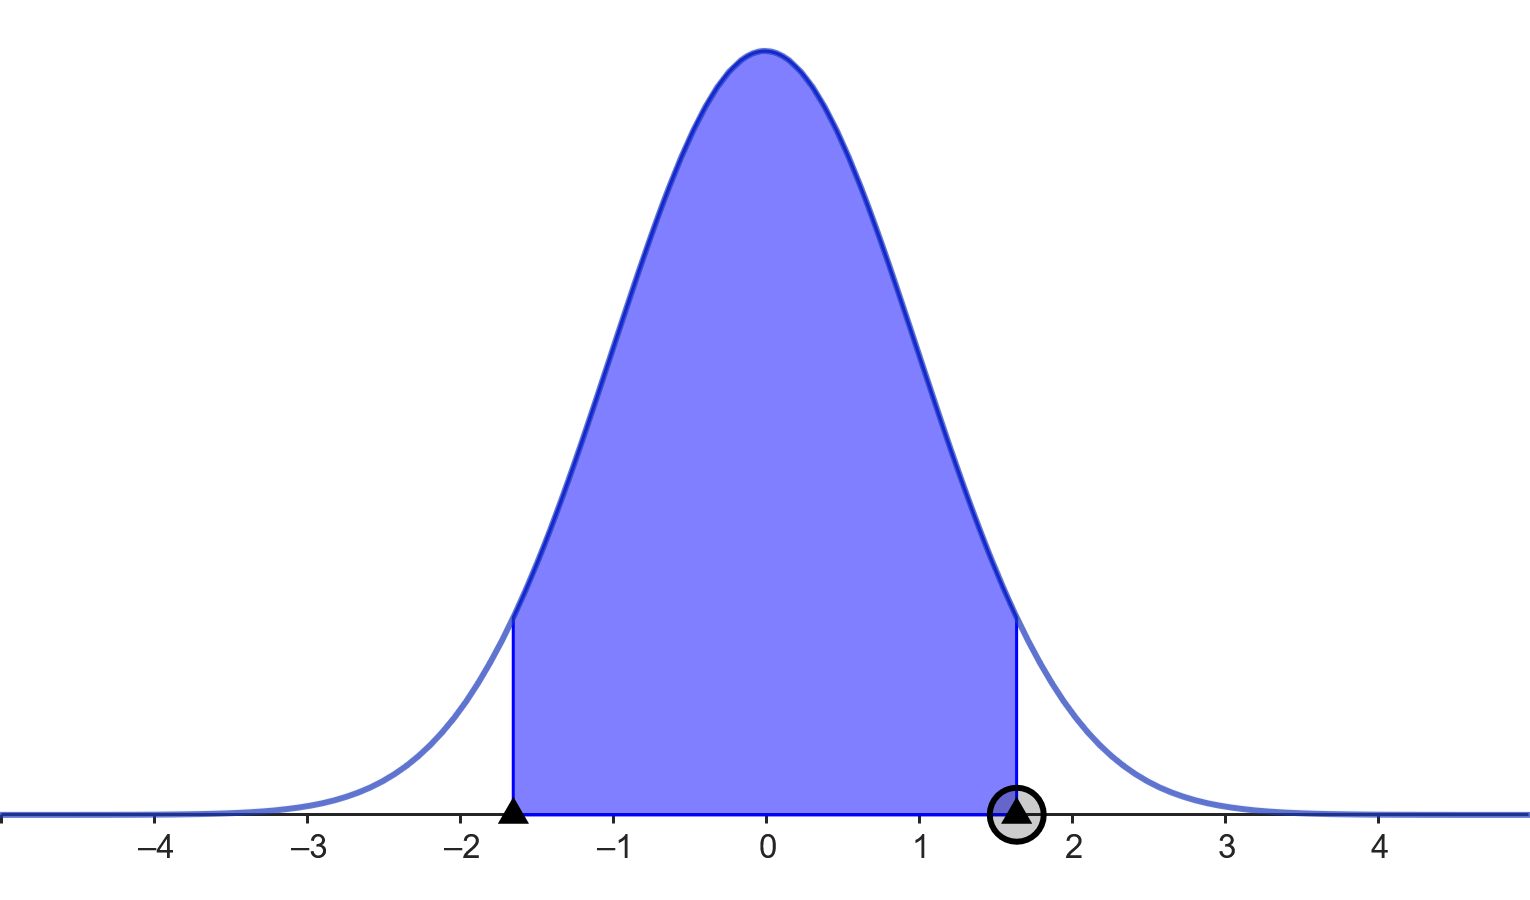
\includegraphics[width=8cm]{Bilder/geogebra-export.png}
  \centering
  \cite{graph_normalverteilung}
\end{figure}

